\begin{figure}[H]
\centering

\begin{minipage}{0.48\textwidth}
\centering
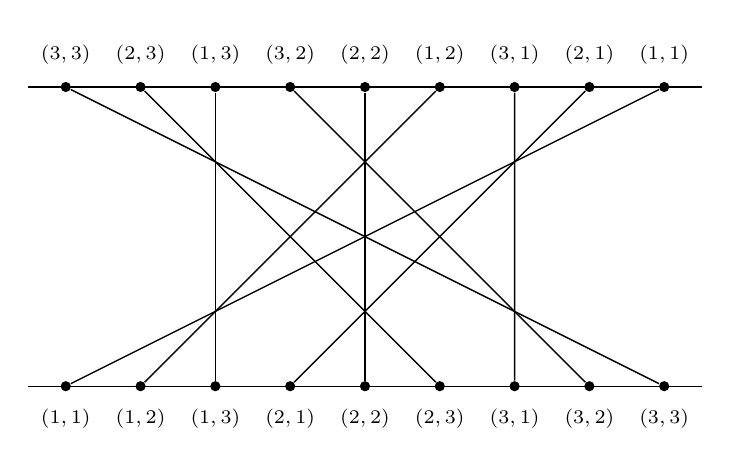
\begin{tikzpicture}[
    scale=0.95,
    every node/.style={circle, fill=black, inner sep=1.3pt},
    edge/.style={line width=0.5pt},
    lab/.style={draw=none, fill=none, inner sep=0pt, font=\scriptsize}
]
\draw[line width=0.5pt] (0.5,0) -- (9.5,0);
\draw[line width=0.5pt] (0.5,4) -- (9.5,4);

\node (b11) at (1,0) {};
\node (b12) at (2,0) {};
\node (b13) at (3,0) {};
\node (b21) at (4,0) {};
\node (b22) at (5,0) {};
\node (b23) at (6,0) {};
\node (b31) at (7,0) {};
\node (b32) at (8,0) {};
\node (b33) at (9,0) {};

\node (t33) at (1,4) {};
\node (t23) at (2,4) {};
\node (t13) at (3,4) {};
\node (t32) at (4,4) {};
\node (t22) at (5,4) {};
\node (t12) at (6,4) {};
\node (t31) at (7,4) {};
\node (t21) at (8,4) {};
\node (t11) at (9,4) {};

\draw[edge] (b11) -- (t11);
\draw[edge] (b12) -- (t12);
\draw[edge] (b13) -- (t13);
\draw[edge] (b21) -- (t21);
\draw[edge] (b22) -- (t22);
\draw[edge] (b23) -- (t23);
\draw[edge] (b31) -- (t31);
\draw[edge] (b32) -- (t32);
\draw[edge] (b33) -- (t33);

\node[lab, below=2pt] at (b11) {$(1,1)$};
\node[lab, below=2pt] at (b12) {$(1,2)$};
\node[lab, below=2pt] at (b13) {$(1,3)$};
\node[lab, below=2pt] at (b21) {$(2,1)$};
\node[lab, below=2pt] at (b22) {$(2,2)$};
\node[lab, below=2pt] at (b23) {$(2,3)$};
\node[lab, below=2pt] at (b31) {$(3,1)$};
\node[lab, below=2pt] at (b32) {$(3,2)$};
\node[lab, below=2pt] at (b33) {$(3,3)$};

\node[lab, above=2pt] at (t33) {$(3,3)$};
\node[lab, above=2pt] at (t23) {$(2,3)$};
\node[lab, above=2pt] at (t13) {$(1,3)$};
\node[lab, above=2pt] at (t32) {$(3,2)$};
\node[lab, above=2pt] at (t22) {$(2,2)$};
\node[lab, above=2pt] at (t12) {$(1,2)$};
\node[lab, above=2pt] at (t31) {$(3,1)$};
\node[lab, above=2pt] at (t21) {$(2,1)$};
\node[lab, above=2pt] at (t11) {$(1,1)$};

% \node[lab] at (5,-0.8) {bottom order: $(1,1),(1,2),(1,3),(2,1),(2,2),(2,3),(3,1),(3,2),(3,3)$};
% \node[lab] at (5,4.8) {top order: $(3,3),(2,3),(1,3),(3,2),(2,2),(1,2),(3,1),(2,1),(1,1)$};
\end{tikzpicture}
\end{minipage}
\hfill
\begin{minipage}{0.48\textwidth}
\centering
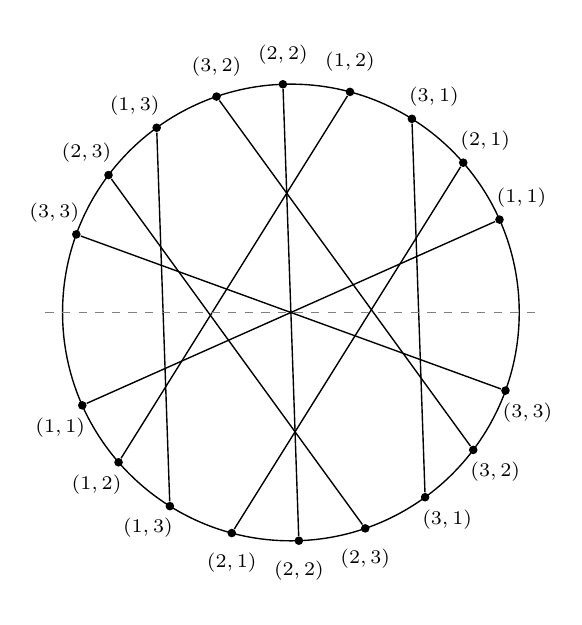
\begin{tikzpicture}[
    scale=1.45,
    every node/.style={circle, fill=black, inner sep=1.1pt},
    edge/.style={line width=0.5pt},
    lab/.style={draw=none, fill=none, inner sep=0pt, font=\scriptsize}
]
\draw[line width=0.5pt] (0,0) circle (2);

\node (u1) at (160:2) {};
\node (u2) at (143:2) {};
\node (u3) at (126:2) {};
\node (u4) at (109:2) {};
\node (u5) at (92:2)  {};
\node (u6) at (75:2)  {};
\node (u7) at (58:2)  {};
\node (u8) at (41:2)  {};
\node (u9) at (24:2)  {};

\node (d1) at (204:2) {};
\node (d2) at (221:2) {};
\node (d3) at (238:2) {};
\node (d4) at (255:2) {};
\node (d5) at (272:2) {};
\node (d6) at (289:2) {};
\node (d7) at (306:2) {};
\node (d8) at (323:2) {};
\node (d9) at (340:2) {};

\draw[edge] (u9) -- (d1);
\draw[edge] (u6) -- (d2);
\draw[edge] (u3) -- (d3);
\draw[edge] (u8) -- (d4);
\draw[edge] (u5) -- (d5);
\draw[edge] (u2) -- (d6);
\draw[edge] (u7) -- (d7);
\draw[edge] (u4) -- (d8);
\draw[edge] (u1) -- (d9);

\node[lab, above left=1pt]  at (u1) {$(3,3)$};
\node[lab, above left=1pt]  at (u2) {$(2,3)$};
\node[lab, above left=1pt]  at (u3) {$(1,3)$};
\node[lab, above=1pt]       at (u4) {$(3,2)$};
\node[lab, above=1pt]       at (u5) {$(2,2)$};
\node[lab, above=1pt]       at (u6) {$(1,2)$};
\node[lab, above right=1pt] at (u7) {$(3,1)$};
\node[lab, above right=1pt] at (u8) {$(2,1)$};
\node[lab, above right=1pt] at (u9) {$(1,1)$};

\node[lab, below left=1pt]  at (d1) {$(1,1)$};
\node[lab, below left=1pt]  at (d2) {$(1,2)$};
\node[lab, below left=1pt]  at (d3) {$(1,3)$};
\node[lab, below=1pt]       at (d4) {$(2,1)$};
\node[lab, below=1pt]       at (d5) {$(2,2)$};
\node[lab, below=1pt]       at (d6) {$(2,3)$};
\node[lab, below right=1pt] at (d7) {$(3,1)$};
\node[lab, below right=1pt] at (d8) {$(3,2)$};
\node[lab, below right=1pt] at (d9) {$(3,3)$};

\draw[dashed, gray] (-2.15,0) -- (2.15,0);

\end{tikzpicture}
\end{minipage}
\caption{A permutation graph representation of $\CGrid_{3\times 3}$ and the equivalent circle graph representation.}
\label{fig:perm-to-circle-cgrid}
\end{figure}